\section{Project overview}
\subsection{Goal and motivation}
Heavy rainfall, strong wind and extreme temperatures can overlap in time or
affect the same area in succession. Our project will integrate reported weather
events, daily measurements, current station observations and official alerts to
help an analyst inspect these combined conditions. The intended analytical output
is a Compound Hazard Index (CHI) per county. It will support monitoring and
correlation; it is not a forecast or an official warning product.

Workshop 1 establishes source access, sample profiles, a common data model and
ingestion contracts. The evidence consists of saved responses and a derived NOAA
sample, inspected in the accompanying executed notebook. Production ingestion,
database implementation and the dashboard belong to later workshops.

\paragraph{Constraints.} Requests must respect usage guidance and provider
terms. NWS requires a User-Agent and retains seven days of station observations;
missing older records cannot be recovered from that endpoint. Storm Events is a
delayed, revisable publication, not a real-time feed; an exact current publication
lag remains to be verified. Preserve source attribution and raw versions.

\subsection{Geographic and temporal scope}
We selected Oklahoma, United States, with counties as the analytical unit.
All four assigned sources cover the study area. A 2024 screening of the same
14 event families returned 2,317 Oklahoma Storm Events rows across all 14 types,
compared with 1,350 Colorado rows across 11 types and 21 Denver-name rows across
six types. Oklahoma also aligns with the captured NWS alerts and offers a useful
mix of flood, wind, heat, cold and winter events.

The historical baseline is 1 January 2010 through 31 December 2025: sixteen
complete calendar years that can be partitioned annually. Current conditions
will use a rolling 24-hour interval ending at an hourly UTC boundary. A separate
seven-day context supports trends and recovery. Seasonal comparisons initially
use the same calendar month across baseline years. These are design choices;
the samples do not establish completeness for all years or all counties.

GHCN station USW00013967 and NWS station KOKC provide the Oklahoma City pilot
evidence. One station cannot represent all Oklahoma counties. Later station
selection will measure element/year completeness, require at least 90\% valid
daily coverage per qualifying year and prefer stations with at least twelve
qualifying years. Counties with insufficient evidence will remain incomplete.

\subsection{Hazard measures and units}
\begin{tabularx}{\textwidth}{lYY}
\toprule Source & Measures & Interpretation \\
\midrule
Storm Events & Event type, magnitude/type, injuries, deaths and damage & Magnitude units depend on the hazard and magnitude type. \\
GHCN-Daily & PRCP (mm), TMAX/TMIN ($^{\circ}$C) in the requested metric response & Daily totals/extrema; preserve measurement and quality flags. \\
NWS observations & Temperature, wind, gust, visibility and other values & Retain each property's unitCode and qualityControl. \\
NWS Alerts & Severity, urgency and certainty & Categorical product attributes, not physical measurements. \\
\bottomrule
\end{tabularx}
These values cannot be added directly. The index will require component-specific
normalization, units and coverage rules.

\section{Functional user and user stories}
The proposed user is a county or regional emergency-management analyst who
reviews observations and warnings, compares conditions with historical records,
and needs to explain the evidence behind a monitoring summary. No stakeholder
interview is claimed in this workshop.

\begin{longtable}{L{1.3cm}L{10.5cm}L{3.1cm}}
\toprule Priority & User story & Verification planned \\
\midrule\endhead
Must & As an analyst, I want to see recent observations, alerts and events by county so that I can review current conditions. & Source/time on map and list. \\
Must & As an analyst, I want to compare measurements with a seasonal baseline so that I can assess unusual conditions. & Baseline, units and window visible. \\
Must & As a reviewer, I want to trace a record to its source and capture so that I can check its provenance. & Source ID, raw hash and retrieval time. \\
Should & As an analyst, I want filters for hazard, time and county so that I can focus on a local situation. & Consistent map/table filters. \\
Should & As an analyst, I want freshness and completeness information so that I can distinguish missing data from quiet conditions. & Health panel with run/state metrics. \\
Could & As an analyst, I want to export filtered evidence so that I can include it in a briefing. & Export retains units and provenance. \\
\bottomrule
\end{longtable}
Prediction, automated emergency recommendations and replacement of official NWS
warnings are excluded. The dashboard and story acceptance tests will be
implemented in subsequent workshops.

\section{Source research and validation}
\subsection{Access and source ownership}
All four sources are operated by NOAA/NCEI or the US National Weather Service.
The historical sources use different access methods: bulk compressed CSV archives
and a parameterized NCEI service. Neither requires an API key for the tested
paths. NWS requires an identifying User-Agent. Endpoints and authoritative
documentation are listed in the references and repository source notes.

The cited NCEI guide supports HTTPS GET queries bounded by station, date,
element and format. No numeric quota was confirmed there: it remains
\emph{to verify}. We will cache partitions and bound retries. NWS documents a
cache-friendly API, required User-Agent and an unpublished numeric rate limit;
honor cache headers and back off after errors. Hourly polling is a team proposal.
Key fields are listed in Section 5.1 and the mapping: event ID/type/time/zone and
damage for NOAA; station/date/elements/flags for GHCN; ID, sent/effective,
severity and areas for alerts; ID/time/station and value/unit/QC for observations.

\begin{tabularx}{\textwidth}{lYYY}
\toprule Source & Access/format & Time coverage and updates & Constraints \\
\midrule
Storm Events & Annual gzip CSV archives & Database records begin in 1950; event-type coverage varies historically; archives can be revised. & Cache archives, preserve version and checksum. \\
GHCN-Daily & NCEI Access Data Service; CSV & Station-specific daily history; daily updates and weekly reconstruction. & Station/year coverage must be measured. \\
NWS Alerts & REST GeoJSON & Operational active/recent alerts; no long-term archive assumed. & Respect NWS request guidance; follow pagination. \\
NWS observations & Station REST GeoJSON & Recent observations; documented seven-day retention and possible delays. & Pagination, optional fields and provider differences. \\
\bottomrule
\end{tabularx}

\subsection{Samples and observed results}
\begin{longtable}{L{2.3cm}L{3.6cm}L{5.2cm}L{3.8cm}}
\toprule Source & Sample & Observed result & Limitation \\
\midrule\endhead
Storm Events & 250 derived Oklahoma rows, 2024; 51 columns & 250 distinct event IDs; source archive contains 69,801 rows; selected Oklahoma filter gives 2,317. & Stratified sample, not representative event frequencies. \\
GHCN-Daily & 365 rows, 2025; 12 columns; USW00013967 & 365 unique dates; no duplicate station/date keys; no null requested measurements; 41 PRCP trace flags. & One station/year only. \\
NWS Alerts & Two empty active polls and 238 recent alerts & 238 unique IDs; 42 null geometries, 42 null ends and 79 null instructions. & Recent sample supplements, but does not replace, active polls. \\
NWS observations & Two KOKC pages of 200 features each & 197 shared IDs unchanged; three entered and three left the bounded page. & Next cursor present; absence is not deletion. \\
\bottomrule
\end{longtable}

The active-alert polls were separated by 5,696 seconds (1 hour 34 minutes
56 seconds); both returned HTTP 200 with zero features. Collection timestamps and
document hashes changed, but no alert-level change could be tested. KOKC polls
were separated by 3,627.404123 seconds. Retained alternative KDEN evidence
contains 96 shared IDs, of which one payload changed. This supports retaining
versions and comparing hashes in addition to identifiers.

The notebook checks schema, null percentages, identifiers, duplicate rows,
timestamp parsing, coordinate ranges and source units. GHCN measurements are
also explored with descriptive statistics, monthly means, a TMAX histogram and
temperature/precipitation boxplots. Points beyond boxplot whiskers are retained:
extreme measurements may be relevant weather observations rather than errors.

\begin{figure}[htbp]\centering
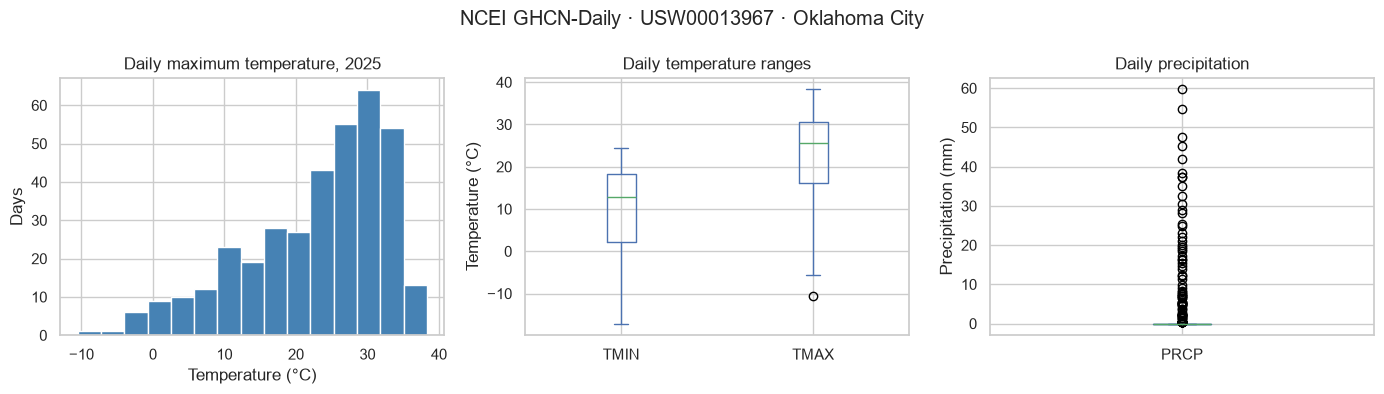
\includegraphics[width=\textwidth]{assets/ghcn_distributions.png}
\caption{Executed notebook output: GHCN daily measurements at USW00013967 in 2025. Precipitation has a different unit and is shown separately.}
\end{figure}

\subsection{Raw evidence and reproducibility}
Saved data and metadata are in \path{workshop_1/samples/}. The evidence register
records capture times, requests, hashes and qualifications. The NOAA CSV is a
deterministic parsed subset; the untouched bulk archive remains in ignored local
raw storage and can be downloaded using the documented script. The notebook
reads saved files and performs eleven checksum comparisons before profiling.
The latest clean-clone execution contains 32 executed code cells and zero error
outputs, using 59 exactly pinned packages and an isolated kernel. A Git
line-ending mismatch in the NOAA subset was corrected without altering its
original registered bytes; the clean run was then repeated successfully.
No new weather request is required to reproduce its computations.

\subsection{Volume estimates}
The 2024 Oklahoma filter contains 2,317 detail rows. Multiplication by sixteen
gives a rough planning screen of 37,072 rows, approximately 41 MB of uncompressed
CSV if row width matches the derived sample. This is not a measured 2010--2025
total. GHCN's 365-row, 54,843-byte pilot response implies roughly 5,840 rows and
0.88 MB for sixteen equally complete years at one station. Leap years, missing
dates, additional stations and changing row widths affect these estimates.
Annual/station-year manifests must measure actual volume before bulk ingestion.

\subsection{Licensing and attribution}
Cite NOAA/NCEI Storm Events with the archive version, access date and selection
filter. No separate dataset license was established by the reviewed evidence.
For GHCN-Daily, use the NCEI Version 3 citation, subset/access information and the
Menne et al. database paper. NCEI provides access and liability terms. NWS states
its data are open/free and generally public domain unless annotated; this does
not grant rights to separately licensed provider content or imply endorsement.
Retain provider/source attribution and review annotations during ingestion.

\section{Data quality and cross-source overlap}
\subsection{Concrete record examples}
The following are integration problems and availability/revision observations;
they are not all provider defects. Q1--Q5 are the five proposed integration
problems; Q6--Q7 are additional availability/sampling examples. The offline submission audit
verifies each cited record claim, not its final rubric acceptance. Exact files,
IDs and interpretation limits appear in the evidence register and audit JSON.
\begin{longtable}{L{1cm}L{4.6cm}L{4.5cm}L{4.8cm}}
\toprule ID & Record & Evidence & Handling proposal \\
\midrule\endhead
Q1 & GHCN USW00013967, 2025-01-05 & PRCP=0.0; attributes T,,W,2400 & Preserve trace flag; distinguish trace from ordinary zero. \\
Q2 & NOAA EVENT\_ID 1155350 & Heavy Snow; CZ\_TYPE=Z; CIMARRON; blank begin latitude/longitude & Retain zone geography and missing point; use a reviewed crosswalk. \\
Q3 & Wind Advisory alert ending in 06189d945720161.001.1 & Null polygon, seven affected-zone URLs & Preserve zones; do not discard for missing polygon. \\
Q4 & KDEN observation 2026-11-04T01:53:00+00:00 & Same ID; temperature changes from null/QC Z to 4.4 $^{\circ}$C/QC V & Compare content hash and retain versions; cause is unproven. \\
Q5 & KOKC 2026-10-31T20:52:00Z & Temperature 16.7 $^{\circ}$C, QC S rather than selected V & Preserve value/QC; exclude from V-only aggregate without declaring the measurement invalid. \\
Q6 & KOKC 2026-11-03T21:52:00Z & Null 24-hour maximum/minimum temperature & Retain missingness and QC; never replace with zero. \\
Q7 & Adjacent KOKC readings 2026-11-03 21:52 and 22:55 UTC & 63-minute interval & Observed sampling limitation, not a proved provider cadence failure. \\
\bottomrule
\end{longtable}
Q3 full ID is \nolinkurl{urn:oid:2.49.0.1.840.0.86cd7f91116ab184a79b0a23e06189d945720161.001.1}.
KDEN/KOKC observation IDs use
\url{https://api.weather.gov/stations/}\emph{station}/observations/\emph{timestamp}.

\subsection{Source-record wind-event candidates}

Five Storm Events records explicitly name the KOKC airport and report measured ASOS wind gusts. They are paired with original GHCN daily WSF5 records for USW00013967, whose returned name and coordinates identify Will Rogers Airport. These are stronger same-weather-episode candidates than generic daily temperature comparisons, not confirmed exact-gust matches or independent sensor validation.

\begin{longtable}{llL{2.4cm}rrr}

\toprule Pair & EVENT\_ID & Local date/time & NOAA (kn) & GHCN (m/s) & $\Delta$ (m/s) \\ \midrule\endhead

WIND-01 & 1170737 & 2024-04-15 15:33 & 50 & 25.5 & -0.22 \\

WIND-02 & 1178563 & 2024-05-06 22:38 & 60 & 30.9 & +0.03 \\

WIND-03 & 1178565 & 2024-05-06 22:45 & 55 & 30.9 & +2.61 \\

WIND-04 & 1178567 & 2024-05-06 22:52 & 56 & 30.9 & +2.09 \\

WIND-05 & 1180427 & 2024-05-19 21:10 & 65 & 33.5 & +0.06 \\

\bottomrule\end{longtable}

\textbf{Time:} NOAA times are CST-6; UTC adds six hours. GHCN has a daily date and null PGTM, so no exact peak timestamp or exact time delta is invented. The same-labelled-local-date rule is provisional; the daily wind boundary is not independently verified.

\textbf{Position:} four event points are about 0.02 km from the returned station point. The High Wind record has zone geography and no point; its narrative names KOKC, and no event coordinate or zero distance is fabricated.

\textbf{Magnitude/identifier:} NOAA measured gusts (MG) in knots convert using 0.5144444444 m/s per knot. GHCN metric WSF5 is fastest 5-second wind, not an identical gust definition. $\Delta$ is GHCN minus converted NOAA. EVENT\_ID differs from station/date/WSF5; all IDs, flags, coordinates, UTC times and file references are in the CSV.

Five pairs use five distinct Storm Events IDs but only three GHCN daily records and three labelled dates. Three May 6 gust reports share one daily summary and may describe one episode. The products can share ASOS reporting lineage. The guide asks for candidate record pairs, not five independent episodes; under that interpretation these are the five proposed overlap examples. Professor acceptance and exact-event equivalence are not asserted.

Full evidence: \path{workshop_1/samples/candidate_pairs/historical_wind_candidate_pairs.csv}; the NOAA file is a checksum-linked parsed subset of the saved archive, and GHCN CSV is the unchanged newly captured response.

\subsection{Supplementary daily temperature comparisons}

One authorized NCEI capture supplies daily summaries for 2026-10-31 through 2026-11-05. Saved KOKC pages are deduplicated by observation ID; conflicting versions would be excluded. We assume fixed CST days (UTC minus six hours), from 06:00Z to the next 06:00Z, as specified for this review. Provider daily boundaries and station equivalence have not been independently established.

The proposed sampling-coverage rule requires at least 48 valid temperatures and no gap, including day edges, greater than 70 minutes. Only unitCode wmoUnit:degC and QC V are accepted. This is a screening criterion, not proof that every continuous daily extreme was observed. One non-V temperature was excluded; no null temperatures or conflicting IDs were found in the combined saved pages.

October 31, November 1, 3 and 4 qualify; November 2 is excluded for a 75-minute gap and November 5 is partial. Precipitation is not aggregated because overlapping windows and missing observations prevent a reliable total. Official 24-hour max/min fields from NWS are not used.

\begin{longtable}{llL{2cm}rrrr}

\toprule Date & Element & UTC window & N & GHCN ($^{\circ}$C) & KOKC ($^{\circ}$C) & $\Delta$ ($^{\circ}$C) \\

\midrule\endhead

2026-10-31 & TMAX & 06:00--06:00 & 116 & 17.8 & 17.2 & -0.6 \\

2026-10-31 & TMIN & 06:00--06:00 & 116 & 15.6 & 15.6 & +0.0 \\

2026-11-01 & TMAX & 06:00--06:00 & 130 & 22.8 & 22.0 & -0.8 \\

2026-11-01 & TMIN & 06:00--06:00 & 130 & 16.1 & 16.0 & -0.1 \\

2026-11-03 & TMAX & 06:00--06:00 & 131 & 17.8 & 17.2 & -0.6 \\

2026-11-03 & TMIN & 06:00--06:00 & 131 & 9.4 & 10.0 & +0.6 \\

2026-11-04 & TMAX & 06:00--06:00 & 133 & 21.1 & 21.0 & -0.1 \\

2026-11-04 & TMIN & 06:00--06:00 & 133 & 6.7 & 7.0 & +0.3 \\

\bottomrule\end{longtable}

Each row compares one date/element, not a distinct weather episode. GHCN identifiers use \path{USW00013967/date/element}; NWS identifiers use \path{KOKC/date/element} plus first, last and extreme observation IDs in the submitted CSV. GHCN flags and NWS QC are preserved there. The GHCN coordinates are taken from the saved 2025 station metadata because this new response does not include coordinate columns; that historical position is not a newly verified station location.

The station-point distance computed from those saved coordinates and the extreme observation point is about 1.29 km. Coordinate proximity does not establish equivalent sensors, exposure or reporting practice. Time differences are daily-summary versus point-sampling granularity; the CSV retains the exact extreme timestamps and seconds from the assumed day boundary.

A sampled KOKC maximum may be lower than a daily GHCN maximum, and a sampled minimum may be higher. Boundary conventions, sampling and station differences can also reverse those differences. These eight rows are candidates, not ground truth. No polygon containment or station equivalence is claimed. Appendix A retains the earlier intra-NWS examples separately.

The NWS side is a derived daily aggregate with a traceable raw extreme observation, not an original daily event record. These eight supplementary comparisons are not counted toward the five primary wind-event candidate examples above and are not eight independent events.

Full comparison and coverage: \path{workshop_1/samples/candidate_pairs/cross_source_candidate_pairs.csv} and \path{daily_coverage.csv}.


\section{Canonical data contract}
\subsection{Common field mapping}
The separately submitted \path{workshop_1/mapping.md} provides the detailed table.
\begin{longtable}{L{2.1cm}L{3cm}L{3cm}L{3cm}L{3.8cm}}
\toprule Field & Storm Events & GHCN & Alerts & Observations \\
\midrule\endhead
event\_id & Source + EVENT\_ID & Station / date / element & Source + alert ID & Source + observation ID \\
source & NOAA catalog key & NCEI catalog key & NWS Alerts key & NWS station key \\
event\_type & EVENT\_TYPE & Element code & properties.event & Observation/element type \\
timestamp & Begin time + CZ\_TIMEZONE & Daily DATE & effective; retain other times & properties.timestamp \\
latitude / longitude & Begin point if present & Station point & Original polygon/zones retained & Feature point \\
severity & Hazard magnitude/type & Measurement + unit & CAP category & Measurement + unit/QC \\
raw\_reference & Archive, record, checksum & Capture, station/date, checksum & Poll, ID, checksum & Poll, ID, checksum \\
\bottomrule
\end{longtable}
Normalize instants to UTC and coordinates to WGS84 decimal degrees. GHCN daily
dates retain their daily temporal resolution; they must not become invented
observation instants. Point fields remain nullable for area-based alerts/events,
with geometry stored separately. Domain values and categorical severities remain
source-qualified. A derived internal ID and content hash distinguish identity
from revisions.

\paragraph{Conversion rules.} Parse NOAA damage as nonnegative decimal plus
K/M/B multiplier (thousands/millions/billions of USD); for example the rule
\texttt{10.00K} gives 10,000 USD, without claiming it occurs in the sample.
Blank/unknown codes remain null or flagged. Read the fixed offset in
CZ\_TIMEZONE: CST-6 adds six hours to local standard time, with date rollover;
do not silently apply daylight saving. Convert NWS unitCode values by dimension:
km/h divided by 3.6 gives m/s, knots multiply by 0.5144444444, Fahrenheit converts
as $(F-32)5/9$, metres of precipitation multiply by 1,000 for mm, and Pa divide
by 100 for hPa. Retain raw units, values, QC and accumulation duration; unknown
codes require review. The full conversion dictionary is in the mapping table.

\subsection{Conceptual entities and relationships}
The common model includes source, ingestion\_run, ingestion\_state, event,
event\_group and rejected\_record. Source-specific domain tables reference the
canonical event. Raw captures retain retrieval metadata and checksums. The
geographic extension stores region, station and source geography with versioned
station/county and zone/county relations.

\begin{figure}[htbp]\centering
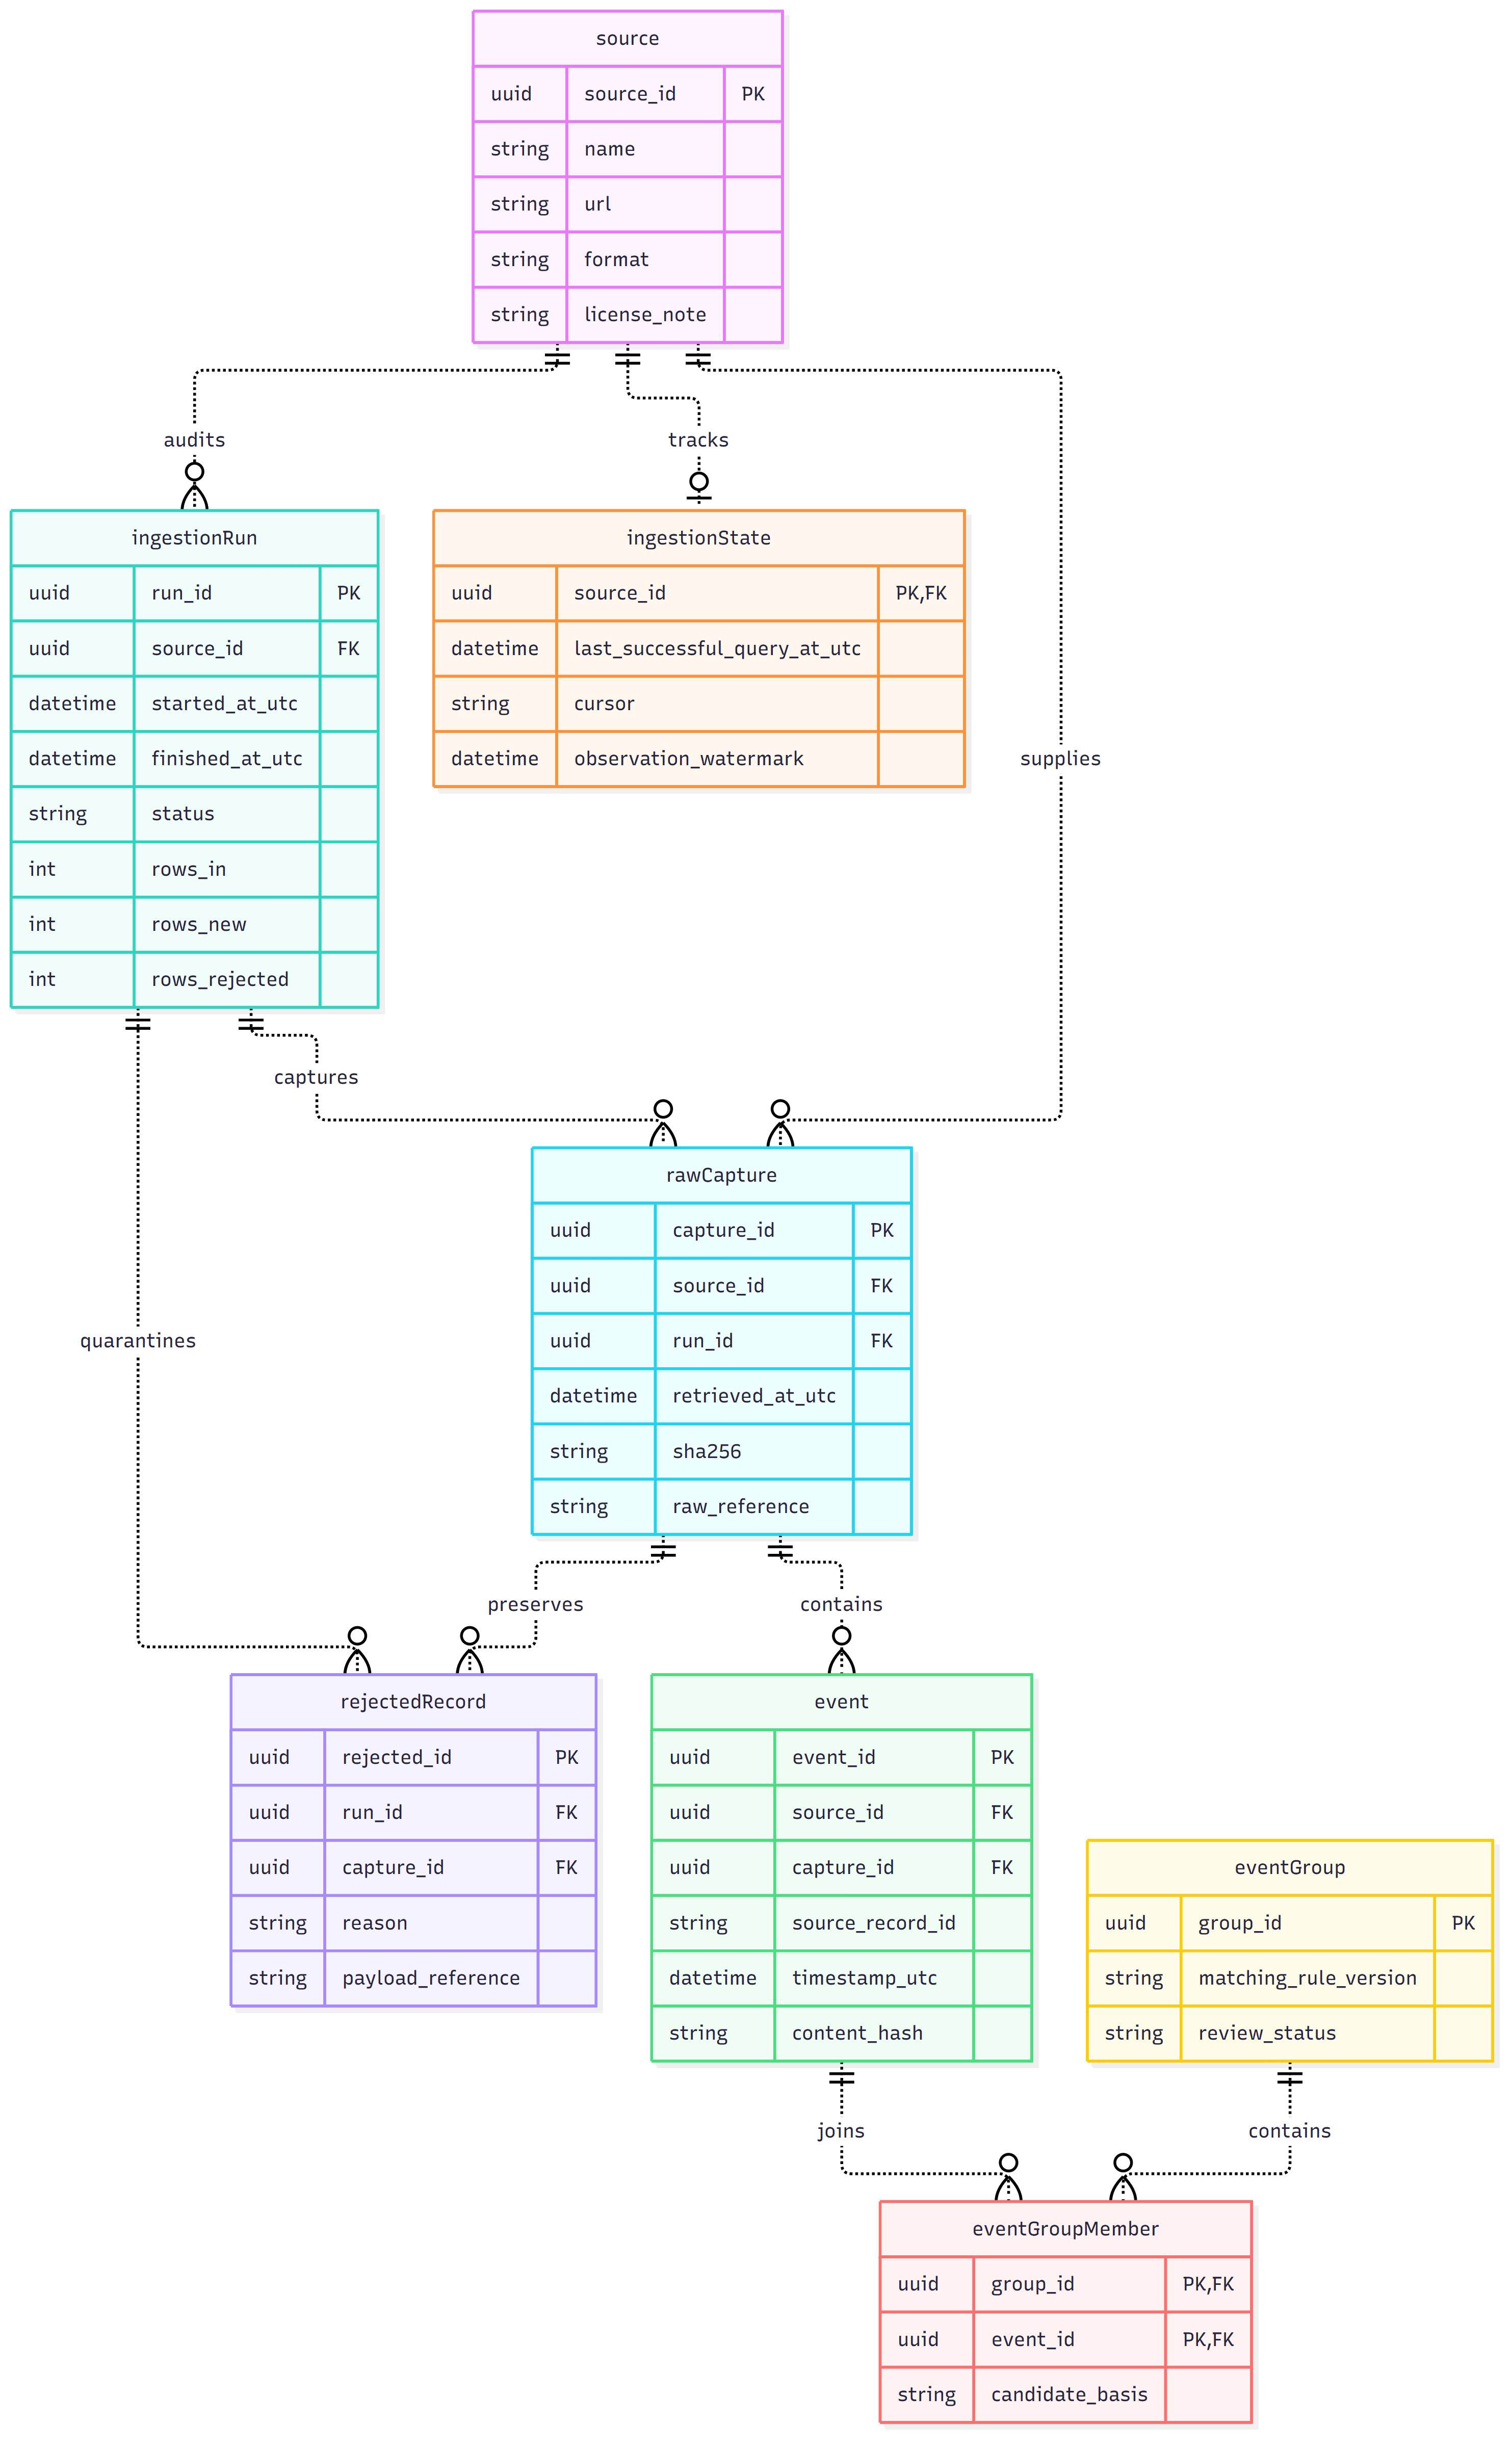
\includegraphics[width=\textwidth,height=0.7\textheight,keepaspectratio]{assets/er-core.png}
\caption{Mermaid ER core with PK/FK and cardinalities. Proposed field types and constraints require SQL implementation review.}
\end{figure}

\begin{figure}[htbp]\centering
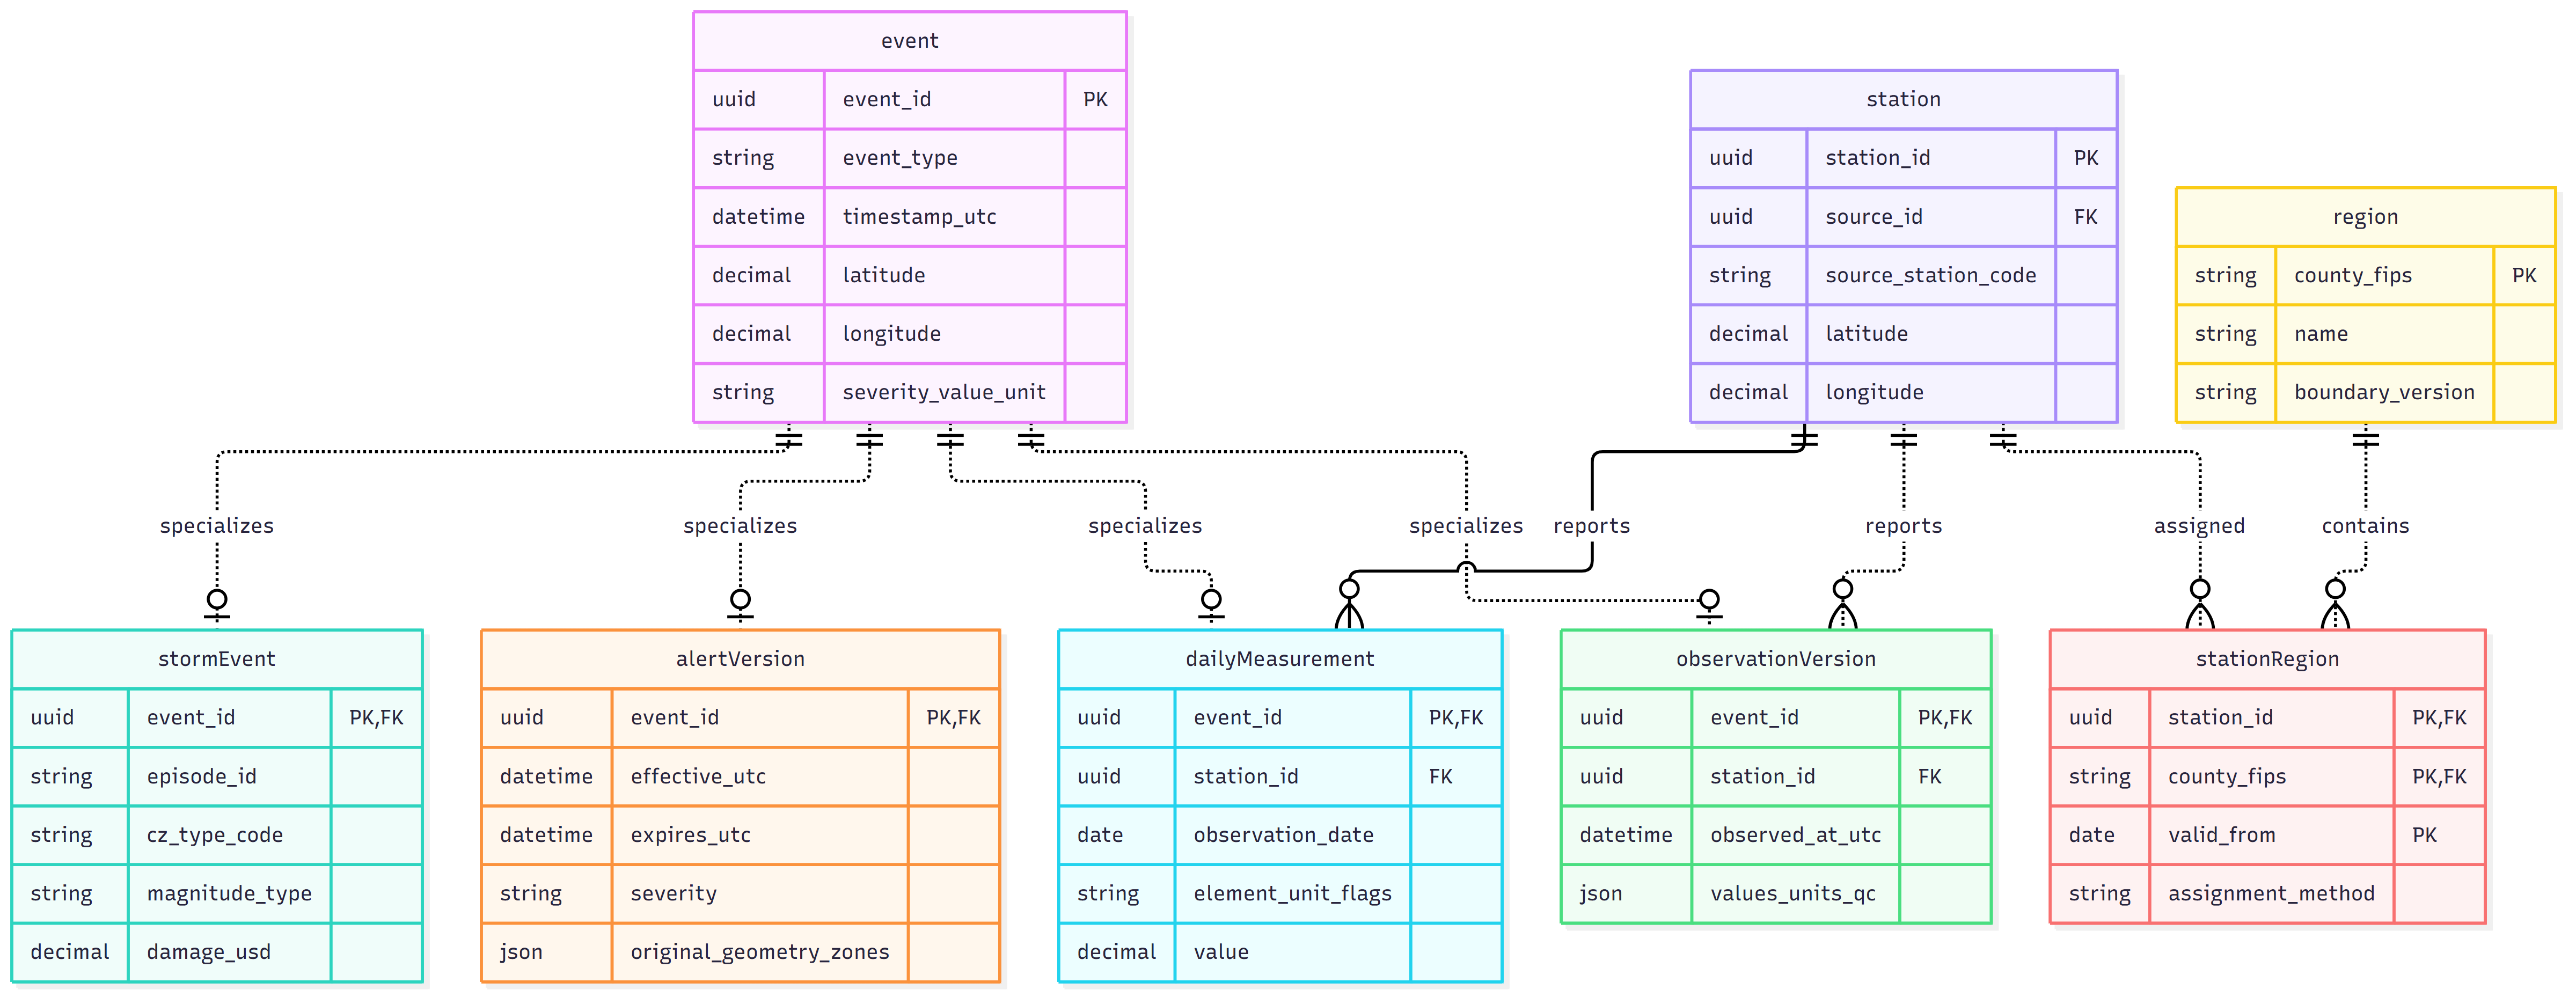
\includegraphics[width=\textwidth,height=0.7\textheight,keepaspectratio]{assets/er-domain.png}
\caption{Mermaid domain extension: event subtypes, measurements and station/county assignment. Daily dates retain their resolution; canonical timestamp may be null for daily records.}
\end{figure}
Editable sources are \path{docs/architecture/workshop-1-core.mmd} and
\path{docs/architecture/workshop-1-domain.mmd}. Domain rows are mutually exclusive
subtypes of a source record; station/source identity and content versions remain
distinct. Further zone/polygon crosswalk fields are detailed in the repository
model and mapping.

The course's \texttt{watermark} maps to \texttt{observation\_watermark} for
station records and to the successful-query checkpoint for active-alert
snapshots. Its \texttt{last\_success} maps to
\texttt{last\_successful\_query\_at\_utc}, advanced only after commit.
Figure 3 extends \texttt{event} with latitude, longitude and severity/value/unit;
these are the same conceptual entity as the core figure, not a second table.

Storm Events preserve episode, magnitude/type, damage and impact fields. Daily
measurements preserve element, value, unit and M/Q/S flags. Alerts preserve CAP
attributes, temporal fields and affected areas. Station observations preserve
value/unit/QC and per-observation geometry. Event groups record the matching rule
version and review status. Records without defensible coordinates keep their
source geography; downstream mandatory-location failures enter quarantine.

\FloatBarrier
\section{Ingestion contracts}
\subsection{Shared recovery rule}
Persist raw bytes and request metadata before parsing. Stage records, validate,
then atomically commit canonical rows, rejects, run metrics and checkpoint.
Advance state only after successful commit. Retry failed partitions/windows using
stable keys and hashes. Keep raw versions for replay and audit.

\begin{longtable}{L{2.1cm}L{4.4cm}L{4.4cm}L{4cm}}
\toprule Source & Historical/partition strategy & Incremental/checkpoint proposal & Key and recovery \\
\midrule\endhead
Storm Events & Cache annual gzip CSV; select Oklahoma hazard families. Compare archive version/checksum on refresh. & Completed archive-year manifest, not a row-level live watermark. & Source/year/EVENT\_ID plus content hash; retry incomplete year. \\
GHCN & Station/year CSV; select qualifying Oklahoma stations and elements. & Completed station/year manifest; recheck partitions for documented revisions. & Raw station/date; normalized station/date/element; retry partition. \\
NWS Alerts & Saved polls form a local archive; recent endpoint is not a durable historical source. & Hourly full snapshot. Operational watermark: last successful query timestamp in UTC, committed with the snapshot. & Alert ID + hash; retain sent/effective per record; no source-side record watermark; absence does not prove deletion. \\
NWS stations & Backfill only within available retention; do not substitute for GHCN history. & Proposed hourly poll, one-hour overlap and daily seven-day reconciliation per station. & Observation ID + hash; follow pagination; retain prior successful state on failure. \\
\bottomrule
\end{longtable}
Schedules and overlap windows are project proposals. Request cost, query support
and statewide coverage must be tested in implementation. The station overlap
accounts for documented arrival delays but does not guarantee detection of every
revision. Preserve observation and retrieval times separately. Rate-limit errors
require timeouts, bounded retries/backoff and source-status logging.

\section{Preliminary Compound Hazard Index}
The five components are flood, wind, heat, cold and winter weather. Candidate
inputs include PRCP and flood alerts; wind/gust and wind events; TMAX/current
temperature and heat alerts; TMIN/current temperature and cold alerts; and winter
event/alert evidence. Historical measurements provide seasonal context, while
reported impacts provide contextual validation. Exact field mappings and
normalization thresholds remain part of later empirical validation.

\begin{samepage}
For component scores $s_h\in[0,1]$, nonnegative weights with $\sum_h w_h=1$, and
configured interaction pairs $\mathcal{P}$, the preliminary rule is
\begin{align*}
B &= \sum_h w_hs_h, &
P &= \max_{(i,j)\in\mathcal{P}}\min(s_i,s_j),\\
\mathrm{CHI} &= 100\min(1,B+\beta P).
\end{align*}
\end{samepage}
Initial parameters are $w_h=0.20$ and $\beta=0.20$, with $P=0$ if no pair is
configured. These are starting parameters, not validated hazard importance.
No interpretation bands are claimed. Missing or stale required components
suppress the total and display an incomplete status; an outage must not appear
as zero hazard. Validation will compare selected documented historical episodes,
seasonal distributions, single versus combined conditions, and sensitivity to
weights/interaction strength. Version parameters and assess false associations,
coverage and geographic uncertainty before interpreting results.

\section{Architecture proposal}
\begin{figure}[htbp]\centering
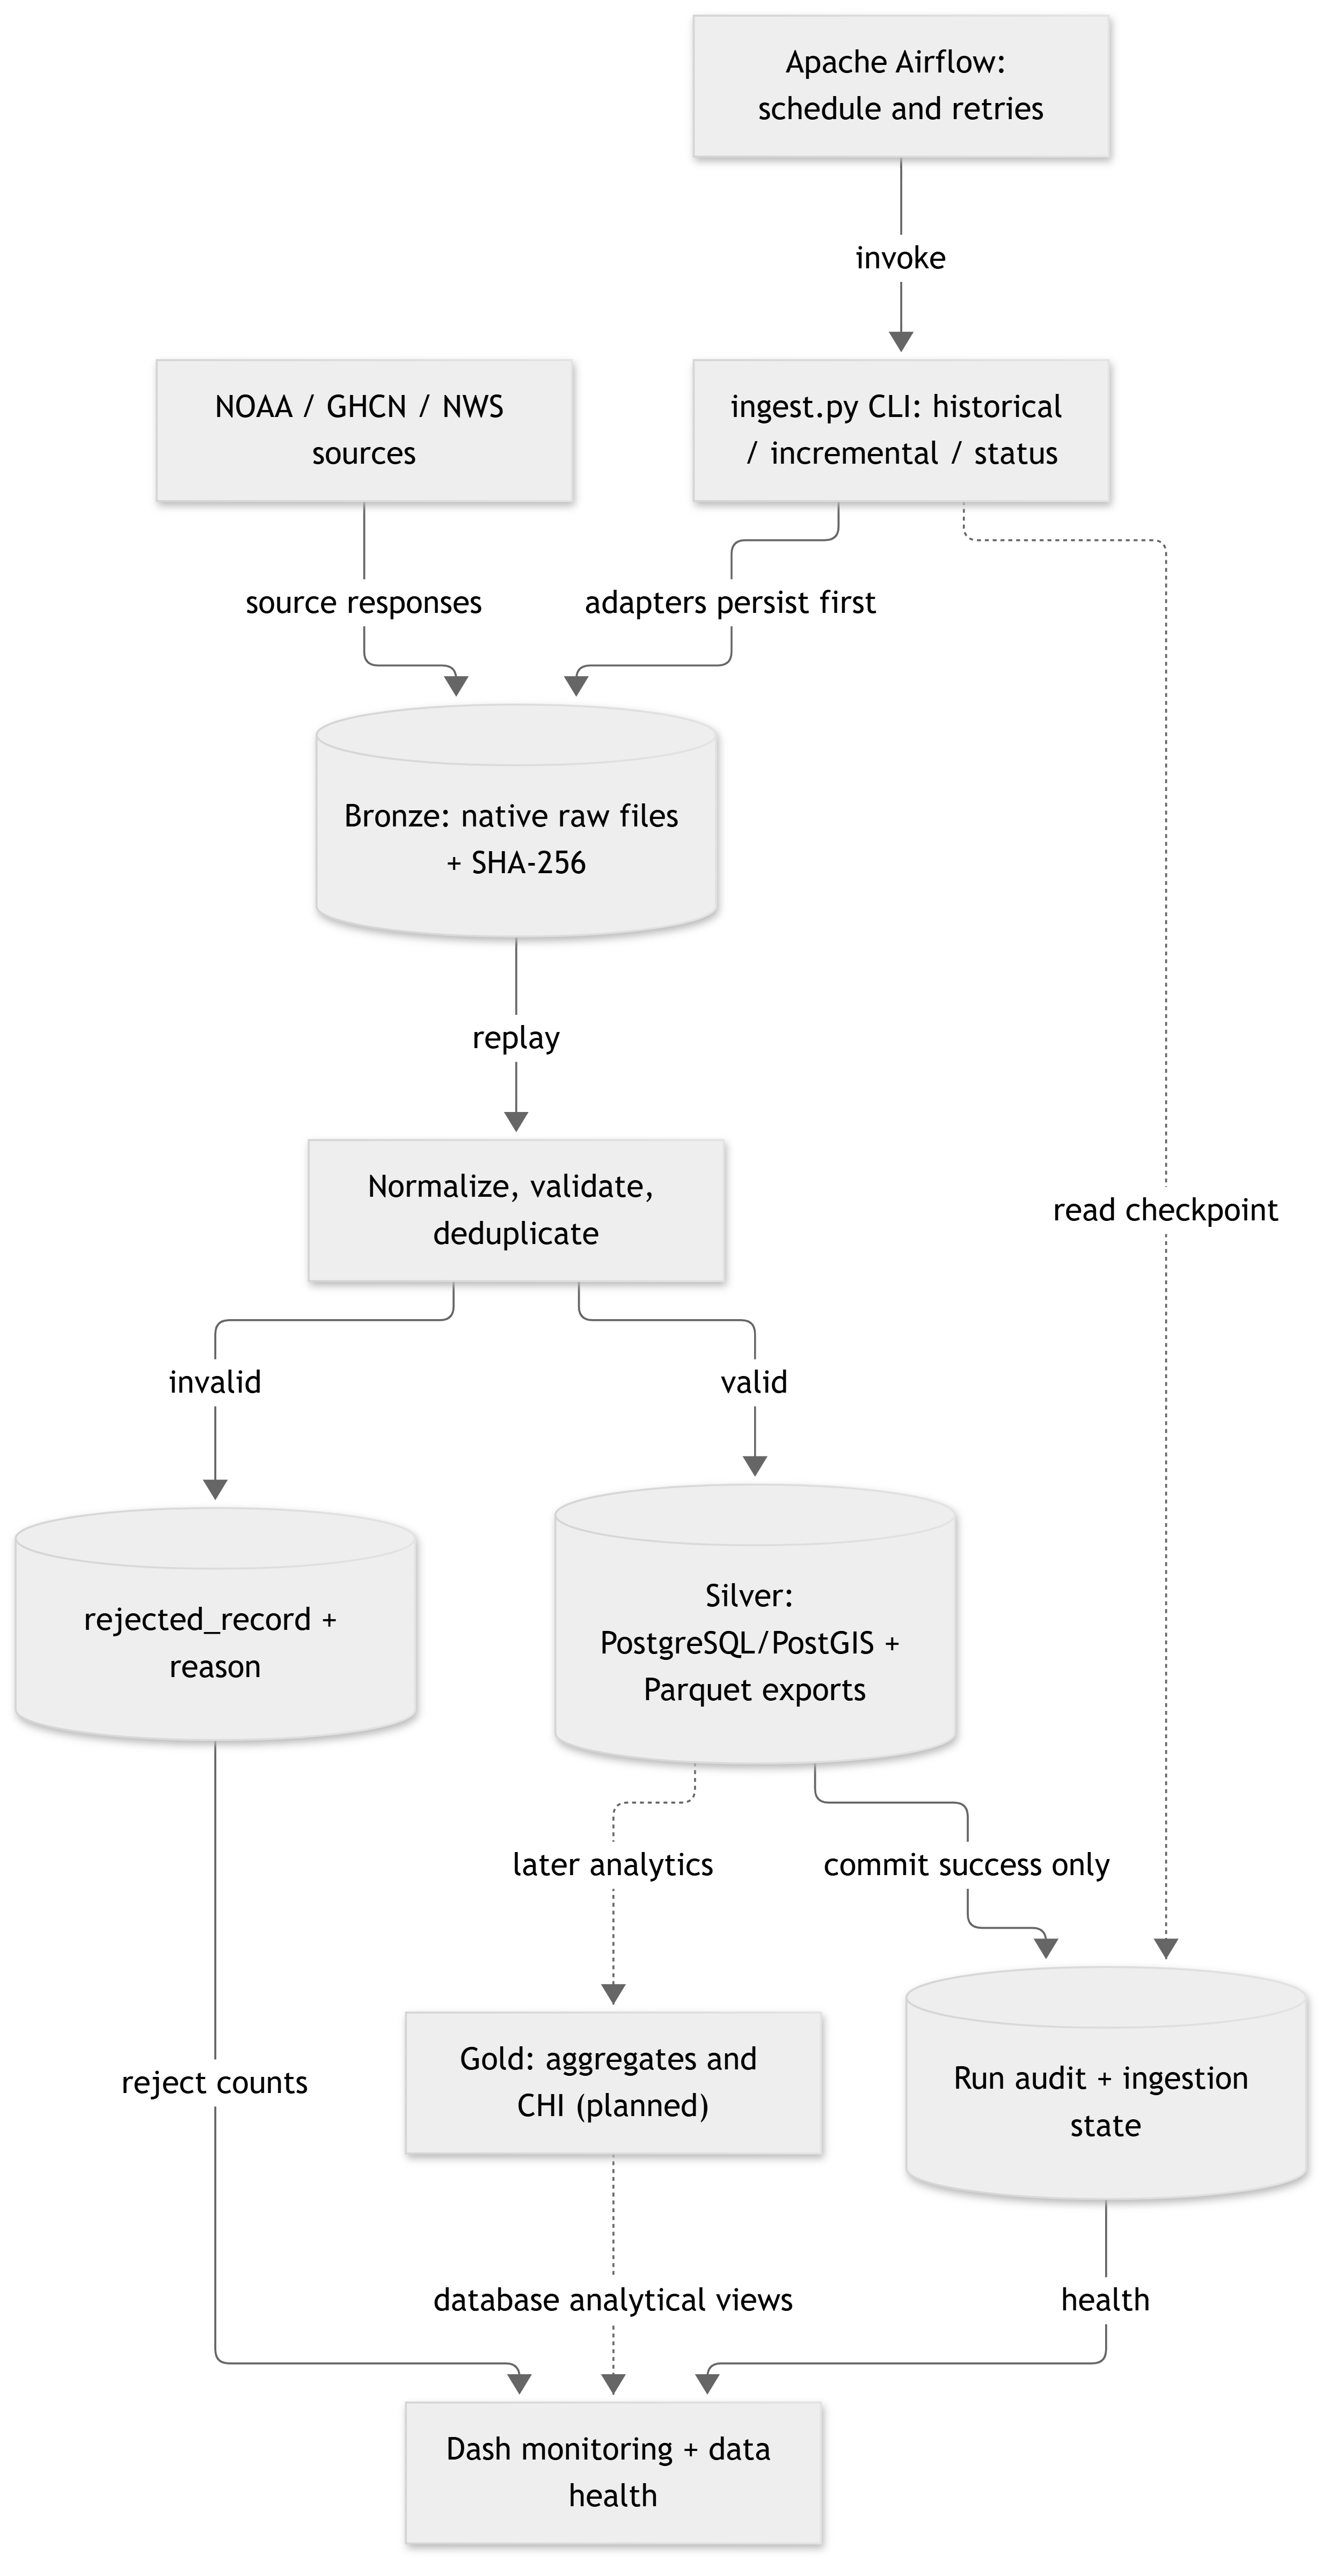
\includegraphics[width=\textwidth,height=0.46\textheight,keepaspectratio]{assets/er-pipeline.png}
\caption{Planned Bronze/Silver/Gold architecture with Apache Airflow, quarantine, canonical storage and committed state. Dashed analytics links belong to later workshops.}
\end{figure}
Editable source: \path{docs/architecture/workshop-1-pipeline.mmd}. The team selects
Apache Airflow for orchestration and PostgreSQL/PostGIS for canonical storage.
Following the course's Airflow/PostgreSQL guide, the design distinguishes three
layers. \textbf{Bronze} retains source-native CSV/gzip or JSON/GeoJSON bytes,
request metadata and SHA-256; a JSON conversion is a derivative, not the original
response. \textbf{Silver} contains normalized, validated records in the canonical
database and traceable Parquet exports. Invalid records enter quarantine rather
than disappearing. \textbf{Gold} will contain temporal/geographic aggregates and
CHI outputs in later workshops; the dashboard will read database analytical views
and health metrics.

The guide demonstrates PostgreSQL Silver and Parquet Gold; the standalone
Workshop 2 handout requests Parquet Silver. The proposed Silver export supports
that artifact without replacing the canonical database. Export publication follows
a successful database commit and retains source/run references. The common CLI
exposes historical, incremental and status modes; configuration stays outside
code and secrets in environment variables. These are design choices, not services
or layer outputs already implemented in Workshop 1. Course reference:
\href{https://github.com/EngAndres/ud-public/blob/main/courses/data-analysis-programming/guides/Airflow-PostgreSQL-ETL.pdf}{Airflow and PostgreSQL ETL Pipeline guide}.

\FloatBarrier
\section{Risks, limitations and next steps}
\begin{tabularx}{\textwidth}{YY}
\toprule Risk & Mitigation \\
\midrule
Source outage, rate limits or schema changes & Cache raw responses, retry with backoff, validate schema and expose failures. \\
Pilot station mistaken for statewide coverage & Measure station/year completeness and expose uncovered counties. \\
Delayed, missing or revised measurements & Preserve source/retrieval times, QC and payload versions. \\
Ambiguous points, zones and polygons & Version geographic crosswalks and retain allocation confidence. \\
Historical volume underestimated & Measure each partition and avoid repeated bulk downloads. \\
License/provider attribution uncertainty & Retain source metadata and review provider annotations/terms. \\
Unsupported precision in CHI & Publish formula, coverage and sensitivity; avoid predictive claims. \\
\bottomrule
\end{tabularx}
Next steps are to review the contracts/mapping, measure statewide station coverage
and partitions, implement historical ingestion with quarantine/idempotency, then
incremental state and matching. The eight daily temperature candidates are not
ground truth labels; Appendix A retains the five intra-NWS examples separately.
The final SQL types, NOAA timezone lookup and geographic boundary
versions remain implementation decisions.

\section{Submission artifacts and reproducibility}
\begin{tabularx}{\textwidth}{lY}
\toprule Artifact & Repository location \\
\midrule
Report source & \path{workshop_1/report/main.tex} and related files \\
Executed notebook & \path{notebooks/01_source_profiling.ipynb} \\
Canonical mapping & \path{workshop_1/mapping.md} \\
Samples and metadata & \path{workshop_1/samples/} \\
Evidence index & \path{deliveries/01-workshop-1/EVIDENCE_REGISTER.md} \\
Dependencies & \path{requirements-workshop1.in} and \path{requirements-workshop1.lock} \\
\bottomrule
\end{tabularx}
Repository: \url{https://github.com/KevMasMas/multi-hazard-weather-monitoring/tree/workflow-1}.
Open the notebook from a clone with the documented dependencies. It uses relative
paths and saved evidence. Re-execute all cells before reviewing outputs. The CLI,
source package, SQL, dashboard and test directories are scaffolds required by the
course; they do not establish implemented pipeline behavior.

\section*{References}
\addcontentsline{toc}{section}{References}
\begin{enumerate}
\item Sierra, C. A. Data Analysis Programming, 2026-II: Course Project, Team Distribution and Workshop 1. \url{https://github.com/EngAndres/ud-public/tree/main/courses/data-analysis-programming/project}
\item NOAA/NCEI. Storm Events Database and bulk archives. \url{https://www.ncei.noaa.gov/stormevents/}; \url{https://www.ncei.noaa.gov/pub/data/swdi/stormevents/csvfiles/}
\item NOAA/NCEI. Storm Data Bulk CSV Format. \url{https://www.ncei.noaa.gov/pub/data/swdi/stormevents/csvfiles/Storm-Data-Bulk-csv-Format.pdf}
\item NOAA/NCEI. GHCN-Daily Version 3 metadata and citation. \url{https://www.ncei.noaa.gov/access/metadata/landing-page/bin/iso?id=gov.noaa.ncdc:C00861}
\item Menne, M. J., et al. (2012). An overview of the Global Historical Climatology Network-Daily Database. Journal of Atmospheric and Oceanic Technology, 29, 897--910. \url{https://doi.org/10.1175/JTECH-D-11-00103.1}
\item NOAA/NCEI. GHCN-Daily README. \url{https://www.ncei.noaa.gov/pub/data/ghcn/daily/readme.txt}
\item NOAA/NCEI. Access Data Service documentation. \url{https://www.ncei.noaa.gov/support/access-data-service-api-user-documentation}
\item National Weather Service. API and alert documentation. \url{https://www.weather.gov/documentation/services-web-api}; \url{https://www.weather.gov/documentation/services-web-alerts}
\item National Weather Service. Disclaimer and use of information. \url{https://www.weather.gov/disclaimer}
\end{enumerate}
